\documentclass[11pt]{article}
\usepackage[margin=.94in]{geometry}
\usepackage{amsmath,amssymb,amsthm,booktabs,graphicx}
\usepackage[colorlinks=true,linkcolor=blue,urlcolor=blue,citecolor=blue]{hyperref}
\usepackage{lmodern,microtype,float}
\newtheorem{theorem}{Theorem}
\newtheorem{lemma}[theorem]{Lemma}
\newtheorem{corollary}[theorem]{Corollary}
\newcommand{\dd}{\,\mathrm d}
\newcommand{\e}{\mathrm e}
\newcommand{\ii}{\mathrm i}
\newcommand{\ord}{\operatorname{ord}}
\newcommand{\J}{\mathcal J}
\newcommand{\K}{\mathcal K}
\newcommand{\PP}{P_x}
\hypersetup{pdftitle={Paired Euler products at the critical line}}
\setlength{\emergencystretch}{2em}
\title{Paired Euler products at the critical line\\[2pt]
\large All-cutoff limits and the signed zero spectrum of the Dirichlet GRH proof}
\author{Research note}\date{25 November 2026}
\begin{document}\maketitle
\begin{abstract}
The deep Riemann hypothesis predicts the behavior of an ordinary partial Euler product at a fixed point of the critical line for every sufficiently large cutoff. We prove an all-cutoff analogue for pairs of ordinary products at offsets of order $1/\log x$. Two offsets whose phases at the cutoff are opposite cancel the uncontrolled prime-sum error. For a real nonprincipal character this gives a single moving-height modulus with an explicit limit, including its prime-square correction. At general fixed height a local mean-square estimate recovers the individual asymptotic on most cutoffs in every one of a family of shrinking logarithmic intervals. We also invert the signed residue formula in the Lean development and recover its modulus and quadratic twist from its aggregated zero spectrum. The external input on zeros is precisely Dirichlet GRH.
\end{abstract}

\section{A pointwise result close to the central point}
For a primitive nonprincipal Dirichlet character $\chi$ put
\[
 P_x(s,\chi)=\prod_{p\le x}(1-\chi(p)p^{-s})^{-1},\qquad u=\log x.
\]
For example, write $\beta(s)=L(s,\chi_4)$ for the Dirichlet beta function,
where $\chi_4(1)=1,\ \chi_4(3)=-1$ on the odd residue classes modulo four. Then
\begin{equation}\label{eq:beta}
 \lim_{x\to\infty}\left|P_x\!\left(\tfrac12+\frac{\pi\ii}{2\log x},\chi_4\right)\right|
 =\beta(\tfrac12)\exp\!\left(\tfrac12\int_1^2\frac{\cos(\pi t/2)}{t}\dd t\right).
\end{equation}
There is no exceptional set in this limit. At height zero the deep Riemann hypothesis (DRH) predicts $P_x(1/2,\chi_4)\to\sqrt{2}\,\beta(1/2)$ for the same sharp cutoff. Conrad isolates the same fixed-height prime-sum obstruction in the proof of Theorem 6.2, equations (6.12)--(6.17), and relates that problem to a prime-sum estimate stronger than the usual pointwise estimate supplied by GRH \cite{conrad,kaneko}. Sheth establishes the predicted fixed-center asymptotic outside a set of finite logarithmic measure \cite{sheth}. Our shift tends to zero at the scale on which the largest prime factors rotate through a fixed angle. It changes the prime-square contribution as well as the endpoint error.

Fix $s_0=1/2+\ii\theta$ and let $m=\ord_{s=s_0} L(s,\chi)$, with $m=0$ at a nonzero value. Define
\begin{gather*}
 A_0=\e^{-m\gamma_E}\frac{L^{(m)}(s_0,\chi)}{m!},\qquad
 \delta=\mathbf1_{\{\theta=0,\ \chi^2\text{ principal}\}},\\
 \J(a)=\int_0^1\frac{1-\e^{-\ii at}}{t}\dd t,\qquad
 \K(a)=\frac12\int_1^2\frac{\e^{-\ii at}}{t}\dd t .
\end{gather*}
All implied constants may depend on the fixed character and $\theta$. We always use $\log P_x$ obtained by summing the absolutely convergent power series of each individual local factor. This convention also defines complex linear combinations of logarithms.

\begin{theorem}[Cancellation at the cutoff]\label{thm:pair}
Let $a_1,\ldots,a_r$ be real and $c_1,\ldots,c_r$ complex. Suppose
$\sum_j c_j\e^{-\ii a_j}=0$ and write $S=\sum_j c_j$.
There is a fixed logarithm $C_0$ of $A_0$ such that, for every real $x$ tending to infinity,
\begin{align}
 \sum_j c_j\log P_x(s_0+\ii a_j/u,\chi)+mS\log u
 \notag\\ = S C_0+\sum_j c_j\bigl(m\J(a_j)+\delta\K(a_j)\bigr)
     +O\!\left(\frac{1}{u}\right).\label{eq:lin}
\end{align}
The error is uniform for bounded offsets and bounded $\sum_j |c_j|$.
For integer $c_j$, exponentiation gives an ordinary product or quotient with an unambiguous limiting constant.
\end{theorem}

Taking offsets $0,\pi$ and both coefficients equal to $1$ gives
\begin{equation}\label{eq:two}
 u^{2m}P_x(s_0,\chi)P_x(s_0+\pi\ii/u,\chi)
 \longrightarrow A_0^2\exp\{m\J(\pi)+\delta[\K(0)+\K(\pi)]\}.
\end{equation}
This contains the actual fixed-height sharp product. Taking offsets $2\pi k,0$ with coefficients $1,-1$ instead gives, for every fixed integer $k$,
\[
 \frac{P_x(s_0+2\pi k\ii/u,\chi)}{P_x(s_0,\chi)}
 \longrightarrow \exp\{m\J(2\pi k)+\delta[\K(2\pi k)-\K(0)]\}.
\]
For a real character at $\theta=0$, the products at opposite offsets are conjugates. Taking offsets $\pm\pi/2$ in Theorem~\ref{thm:pair} gives
\[
 u^m|P_x(1/2+\pi\ii/(2u),\chi)|
 \longrightarrow |A_0|\exp\{m\Re\J(\pi/2)+\Re\K(\pi/2)\}.
\]
The alternating series for $\beta(1/2)$ has positive sum, so $m=0$ in \eqref{eq:beta}. These assertions apply to the original unsmoothed factors at all primes $p\le x$. Their logarithmic combinations implement a weight that vanishes exactly at the endpoint.

\begin{figure}[H]
\centering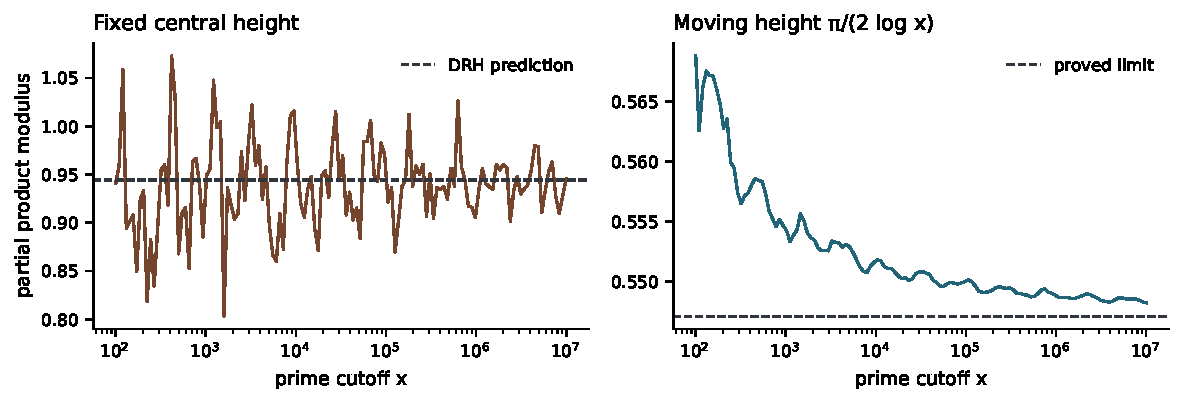
\includegraphics[width=.96\linewidth]{euler_example.pdf}
\caption{Ordinary sharp Euler products for $\chi_4$ at 130 logarithmically spaced cutoffs up to $10^7$. The left reference line is the fixed-center DRH prediction. The right line is the proven limit in \eqref{eq:beta}. Each panel has its own vertical scale. The included script evaluates the constants from a Hurwitz-zeta difference and a real integral.}
\end{figure}

\section{What is imported from the Lean development}
We use the checked nonvanishing theorem for every Dirichlet character in the half-plane $\Re s>1/2$ (with the principal pole excluded) and the critical-strip zero statement. The definitions live in \path{grh/src/Statements.lean}. The exports in \path{grh/src/Main.lean} follow from \texttt{New.grh} \cite{lean}. Sutherland records independent sandboxed builds, statement comparison and kernel checks of both editions at this commit \cite{mit}. We use those records for the upstream artifact. All results introduced in this note have ordinary mathematical proofs.

The internal calculation yields a one-sided bound for a smoothed prime-power sum in one progression with a quadratic twist. Its Mellin poles measure differences of orders of vanishing. The quadratic-twist selection in \path{New/Reduction/Zeros/Criterion.lean} prevents cancellation from hiding a candidate zero in a fixed rectangle. The upper, spanning and lower estimates on integral forms give the determinant inequality in \path{New/Reduction/MainInequality.lean}; \path{New/Reduction/OneSidedBound.lean} converts it into the prime-sum upper bound. The next two sections use the same principle of reading prime weights through the modes they retain: one critical oscillation survives a sharp endpoint, and two appropriately chosen offsets remove it. The analytic proof uses classical explicit formulas together with the exported Dirichlet GRH. Section~\ref{sec:packet} uses the specific signed residues inside the repository itself.

\section{Isolating the endpoint}
Write $\Psi(x)=\sum_{n\le x}\chi(n)\Lambda(n)$ and use $\Lambda$ for the von Mangoldt function. For $v>0$, put
\[
 E(v)=\e^{-s_0 v}\Psi(\e^v),\quad F_0(v)=E(v)+m/s_0,\qquad
 H(v)=\sum_{2\le n\le\e^v}\frac{\chi(n)\Lambda(n)}{n^{s_0}\log n}.
\]
Step functions here use right endpoints. Changing values at jumps has no effect on their integrals.

\begin{lemma}\label{lem:primitive}
The primitive $\int_1^V F_0(v)\dd v$ is bounded for $V\ge1$. There is a number $C_0$ with $\exp C_0=A_0$ such that
\begin{equation}\label{eq:H}
 H(v)=C_0-m\log v+\frac{F_0(v)}v+O(1/v)\qquad(v\ge1).
\end{equation}
\end{lemma}
\begin{proof}
The explicit formula for a primitive nonprincipal character \cite{dav,kouk}, in the sense of distributions on $v\ge1$, is
\begin{equation}\label{eq:explicit}
 E(v)=-\sum_{\rho=1/2+\ii\gamma}
            \frac{\e^{\ii(\gamma-\theta)v}}{\rho}+D(v),
 \qquad D(v)=O_\chi((1+v)\e^{-v/2}).
\end{equation}
Zeros are counted with multiplicity. This is Perron's formula for $-L'/L$ after the shift past the nontrivial zeros. The pole of the Perron kernel at zero, the possible trivial zero there and the remaining negative trivial zeros give the stated $D$. A smooth test in $v$ makes the zero sum absolutely convergent. The $m$ terms at $\gamma=\theta$ give $-m/s_0$. After one integration every remaining coefficient is bounded by $2/|\rho(\gamma-\theta)|$. Their sum converges by the zero count $N(T+1)-N(T)\ll_\chi\log(2+T)$ for $T\ge1$, applied to both signs. This proves the bounded-primitive assertion, also when $\theta$ itself is the ordinate of a multiple zero.

Stieltjes partial summation, starting below $\log 2$, gives an endpoint $E(v)/v$ and an integral with integrand $E(w)(s_0/w+1/w^2)$. The constant mode $-m/s_0$ contributes $-m\log v$ and a constant, because its $1/v$ terms cancel. The integral of $F_0(w)(s_0/w+1/w^2)$ to infinity converges, with tail $O(1/v)$ by integration by parts against its bounded primitive. This gives \eqref{eq:H}, pointwise including jumps, with some $C_0$.

For $h>0$, partial summation and the GRH estimate $\Psi(x)\ll_\chi\sqrt x\log^2(2x)$ give
\[
 h\int_0^\infty H(v)\e^{-hv}\dd v=\log L(s_0+h,\chi).
\]
Indeed the log series agrees with the Euler product in $\Re s>1$ and defines its continued logarithm in $\Re s>1/2$ by locally uniform convergence. The constant and logarithm in \eqref{eq:H} contribute $C_0+m\log h+m\gamma_E$. The other terms have Abel mean $o(1)$ as $h\downarrow0$: the $O(1/v)$ remainder contributes $O(h\log(2/h))$ for small $h$, and the bounded primitive treats $F_0(v)/v$ by integration by parts. Comparing the exponential with $L(s_0+h,\chi)\sim h^m L^{(m)}(s_0,\chi)/m!$ proves the claimed normalization.
\end{proof}

\begin{proof}[Proof of Theorem~\ref{thm:pair}]
Set $W(t)=\sum_j c_j\e^{-\ii a_jt}$. Truncation at prime powers $p^k\le x$ gives exactly
\[
 \int_{0-}^u W(v/u)\dd H(v)
 = W(1)H(u)-u^{-1}\int_0^u H(v)W'(v/u)\dd v .
\]
Put $R(v)=H(v)-(C_0-m\log v)$. Its primitive is bounded on $[0,\infty)$. At zero the logarithm is integrable. For $v\ge1$ the partial summation proof gives the exact identity
\[
 R(v)=F_0(v)/v-\int_v^\infty F_0(w)k(w)\dd w,\qquad k(w)=s_0/w+1/w^2.
\]
The first term has a bounded primitive by Lemma~\ref{lem:primitive}. Integrating the tail from $1$ to $V$ gives
$\int_1^V(w-1)k(w)F_0(w)\dd w+(V-1)\int_V^\infty k(w)F_0(w)\dd w$.
The first term is bounded because $(w-1)k(w)$ is bounded and has integrable derivative. The second uses the $O(1/V)$ tail bound. Hence
$\int_0^u R(v)W'(v/u)\dd v=O(\|W'\|_\infty+\|W''\|_\infty)$
by integration by parts. Substitution of the model $C_0-m\log v$ and integration by parts at zero now give
\begin{align}
 \int_{0-}^u W(v/u)\dd H(v)={}& W(0)(C_0-m\log u)
       +m\int_0^1\frac{W(0)-W(t)}{t}\dd t\notag\\
       &+W(1)R(u)+O_W(1/u). \label{eq:endpoint}
\end{align}
The only uncontrolled pointwise quantity is multiplied by $W(1)$.

The ordinary Euler product also contains terms with $p\le x<p^k$. Terms of order $k\ge3$ have total absolute value $O_W(x^{-1/6})$ for these finite exponential weights, which are bounded for all real arguments. For $p>x^{1/3}$ sum $O(p^{-3/2})$; for $p\le x^{1/3}$ sum the geometric tail starting with its first omitted power, which is $O(x^{-1/2})$ per prime. The square terms contribute
\[
 \frac12\sum_{\sqrt{x}<p\le x}\frac{\chi(p)^2}{p^{1+2\ii\theta}}
                        W(2\log p/u)
 = \frac{\delta}{2}\int_1^2\frac{W(t)}t\dd t+O_W(1/u).
\]
For detail, fixed-modulus prime number theory gives
$\sum_{p\le y}\chi^2(p)\log p=\mathbf1_{\chi^2\ {\rm principal}}y+O_\chi(y/\log^3 y)$; any fixed log saving is available. Partial summation on $[\sqrt x,x]$ makes its error $O_{W,\theta}(1/u)$ or smaller. The main integral before setting $\theta=0$ is $\tfrac12\int_1^2 W(t)\e^{-\ii\theta u t}\dd t/t$; integration by parts gives $O_{W,\theta}(1/u)$ for fixed $\theta\ne0$. Using $W(1)=0$ in \eqref{eq:endpoint} completes the proof.
\end{proof}

\section{Individual products on short logarithmic intervals}
The same calculation identifies what remains when the endpoint is retained.
For a real $a$ let
\[
 B(v,a)=\log P_{\e^v}(s_0+\ii a/v,\chi)+m\log v
          -C_0-m\J(a)-\delta\K(a).
\]
Equation~\eqref{eq:endpoint} gives, uniformly for $|a|\le A$,
\begin{equation}\label{eq:single}
 B(v,a)=\e^{-\ii a}\frac{F_0(v)}{v}
             +O_A(1/v).
\end{equation}

Thus the pointwise convergence of the canonical logarithm at the fixed height is equivalent to $\Psi(x)=o(\sqrt{x}\log x)$ for this character. The factor $\e^{-\ii\theta v}$ has unit modulus. The GRH bound $O(\sqrt{x}\log^2 x)$ leaves one logarithm to save and requires a little-oh at the target scale. The cancellation in Theorem~\ref{thm:pair} removes this entire term for the paired observable.

For a real character and fixed $\theta\ne0$, \eqref{eq:single} at $a=0$ gives a deterministic subsequence of the fixed-height prediction. For $n\ge0$ let
\[
 X_n=\exp((\pi/2+n\pi)/|\theta|).
\]
Since $\Psi(X_n)$ is real and $\exp(-\ii\theta\log X_n)$ is purely imaginary, taking real parts gives
\[
 (\log X_n)^m |P_{X_n}(s_0,\chi)|=|A_0|\bigl(1+O(1/\log X_n)\bigr).
\]
This applies even when $s_0$ is a zero. It controls the modulus along an explicit geometric sequence at the actual fixed height.

For complex as well as real $\chi$, two fixed heights $\theta_1\ne\theta_2$ also give a full complex ratio along prescribed cutoffs. Write $s_j=1/2+\ii\theta_j$, and denote by $m_j,A_j,\delta_j$ the corresponding constants. Set $v_n=2\pi n/|\theta_1-\theta_2|$ and $x_n=\exp(v_n)$. Then
\[
 v_n^{m_1-m_2}\frac{P_{x_n}(s_1,\chi)}{P_{x_n}(s_2,\chi)}
 =\frac{A_1}{A_2}2^{(\delta_1-\delta_2)/2}
   \bigl(1+O(1/v_n)\bigr).
\]
In fact, the two uncontrolled terms contain the same $\Psi(x_n)$ with identical phase $\exp(-\ii\theta_j v_n)$, so they cancel on subtraction. This deduction uses \eqref{eq:single} at $a=0$ separately at the two heights.

\begin{theorem}[Local mean square]\label{thm:ms}
For $U\ge2$, $0<h\le1$, and fixed $A<\infty$,
\[
 \left(\frac1h\int_U^{U+h}\sup_{|a|\le A}|B(v,a)|^2\dd v\right)^{1/2}
 \ll_{\chi,\theta,A}\frac{\log^2(2/h)}{U}.
\]
In particular, if $\log(1/h)=o(\sqrt U)$, the normalized individual products converge to their respective profiles
$A_0\exp\{m\J(a)+\delta\K(a)\}$ in relative logarithmic measure in every such interval, uniformly in bounded $a$. This is a mean-square assertion for logarithms and a convergence-in-measure assertion for products.
\end{theorem}
\begin{proof}
For any finite trigonometric sum $T(v)=\sum_\gamma d_\gamma\e^{\ii\gamma v}$, group frequencies in bins $I_j=[j/h,(j+1)/h)$ and put $b_j=\sum_{\gamma\in I_j}|d_\gamma|$. Then
\[
 h^{-1}\int_U^{U+h}|T(v)|^2\dd v\ll\sum_j b_j^2 .
\]
To see this, majorize the interval indicator by a constant times a Gaussian of width $h$ centered at its midpoint. Its Fourier transform bounds the interaction of bins $j,k$ after division by $h$ by $C\exp(-c(\max\{|j-k|-1,0\})^2)$. Sum using $2b_jb_k\le b_j^2+b_k^2$. No lower bound on gaps between ordinates is needed.

Apply this to \eqref{eq:explicit}, dropping the common unit phase $\e^{-\ii\theta v}$. The sum of absolute coefficients for $|\gamma|\le 1/h$ is $O_\chi(\log^2(2/h))$ by summing unit bins. For the positive tail, each bin $j\ge1$ contains $O_\chi(h^{-1}\log(2+(j+1)/h))$ ordinates. Its total absolute coefficient is at most $C_\chi\log(2+(j+1)/h)/j$. The sum of the squares of these bin bounds is $O_\chi(\log^2(2/h))$, and the negative tail obeys the same estimate. This also gives local $L^2$ convergence of the high-frequency series, identifying its limit with the distribution in \eqref{eq:explicit}. The normalized $L^2$ norm of $F_0$ on the interval is consequently $O_{\chi,\theta}(\log^2(2/h))$. Equation~\eqref{eq:single} proves the stated bound. For each fixed tolerance, Chebyshev's inequality bounds the exceptional fraction by the square of the right-hand side divided by the tolerance squared; continuity of exponentiation near zero transfers this to relative product error.
\end{proof}
For instance $h=\exp(-U^{1/3})$ is admissible. The corresponding interval of prime cutoffs starts at $X=\e^U$ and has length asymptotic to $X\exp[-(\log X)^{1/3}]$. The theorem supplies a vanishing exceptional fraction inside every such interval. A qualitative statement that the global exceptional set has finite logarithmic measure, on its own, does not give this local conclusion.



\section{Recovering the modulus and twist from the signed zero spectrum}
\label{sec:packet}
The residues in \texttt{New.isPolar\_primeRemainder} record only the
difference between two sums of zero multiplicities. Contributions at a common
zero can cancel exactly, and the names of the characters have disappeared.
Nevertheless the signed data determine both arithmetic parameters. The proof
also identifies the limiting oscillations of the prime remainder used in the
Lean argument.

Fix $8\mid q$, $q>0$, and a prime $d\equiv7\pmod 8$ coprime to $q$.
Write $h=\varphi(q)$ and $\eta(n)=(n/d)$. For each $\chi\bmod q$ let
$\chi^*$ be its inducing primitive character. For a real ordinate $\gamma$ put
$\rho_\gamma=1/2+i\gamma$ and set
\[
 m(\gamma)=\frac1h\sum_{\chi\bmod q}
 \left(\operatorname{ord}_{\rho_\gamma} L(s,\chi^*)-
       \operatorname{ord}_{\rho_\gamma} L(s,\chi^*\eta)\right),
 \qquad b_\gamma=\frac{m(\gamma)}{1/4+\gamma^2}.
\]
Removing imprimitive Euler factors preserves orders in the open critical
strip. Thus $b_\gamma$ is precisely the residue in the source. Dirichlet GRH
puts every nontrivial zero in these sums on the specified line.
The input to the inverse problem is the signed coefficient at each frequency,
with coincident frequencies combined.

\paragraph{Recovery theorem.}
The series $F(t)=\sum_\gamma b_\gamma e^{i\gamma t}$ is real, even and
uniformly convergent. Its derivative has a jump $\log d$ at zero. At $\log p$
for every prime $p\nmid qd$ it has a jump precisely if
$p\equiv1\pmod q$ and $\eta(p)=-1$, in which case the jump is
$2\log p/\sqrt p$. Consequently the data $\{(\gamma,b_\gamma)\}$
determine $(q,d)$ even if they have been changed at finitely many frequencies.
More generally, the same reconstruction works after adding any continuously
differentiable function to $F$. It concerns the full infinite spectrum and
does not assert a cutoff at which a finite list determines the parameters.

\paragraph{Proof of the jump formula.}
The classical zero count $N(T)=O_{q,d}(T\log(2+T))$ ensures
$\sum_\gamma |b_\gamma|<\infty$ by partial summation. Both families are closed
under complex conjugation, whence $b_{-\gamma}=b_\gamma\in\mathbb R$.
For a prime power $n=p^k$ let $Q_p=p^{v_p(q)}$, $q^{(p)}=q/Q_p$, and put
\[
 a(p^k)=\frac{1-\eta(p^k)}{\varphi(Q_p)}
               \mathbf 1_{p^k\equiv1\bmod q^{(p)}} .
\]
In distributions on the real line the following identity holds, with
$\delta_u$ a unit point mass at $u$:
\begin{align}
 F''-\tfrac14 F={}&(\log d)\delta_0-
       \frac2h\cosh(t/2)\,dt \notag\\
 &+\sum_{p^k\ge2}\frac{\log p}{p^{k/2}}\,a(p^k)
                     (\delta_{\log p^k}+\delta_{-\log p^k}).
 \label{eq:packet-ode}
\end{align}
Here derivatives are taken in the distributional sense and functions are
identified with their densities. To check the constants, test against
$g\in C_c^\infty(\mathbb R)$ with
$H(u)=\int g(t)e^{iut}\,dt$. The Guinand--Weil explicit formula for a
primitive character of conductor $f$ contributes $\log(f/\pi)g(0)$, the
gamma term for its parity, and a negative sum of prime powers with
coefficients $\Lambda(n)\chi^*(n)/\sqrt n$ at one sign of $\log n$ and
the conjugate coefficients at the other. The primitive principal character
also contributes $H(i/2)+H(-i/2)$ from the poles at $0,1$ of the completed
zeta function. This is the normalization of
A.~Chirre, V.~J.~Pereira J\'unior and D.~de Laat,
\emph{Primes in arithmetic progressions and semidefinite programming},
Math. Comp. 90 (2021), \S2.1,
\href{https://doi.org/10.1090/mcom/3638}{doi:10.1090/mcom/3638}.
Equivalently the formula follows by shifting the contour of the logarithmic
derivative of the completed primitive $L$-function.

As $q>2$, half the characters have each parity. The odd character $\eta$
interchanges the parities. All gamma terms therefore cancel between the two
families. The two conductors for $\chi^*$ and $\chi^*\eta$ are $f$ and
$fd$, since $(f,d)=1$. Only the untwisted family contains the primitive
principal character. At $p^k$ the average of the untwisted primitive
character values is $\mathbf 1_{p^k\equiv1\bmod q^{(p)}}/\varphi(Q_p)$.
Indeed a nonprincipal $p$-component makes the primitive value zero,
and orthogonality over the characters modulo $q^{(p)}$ evaluates the
remaining sum. Multiplication by $1-\eta(p^k)$ gives the displayed $a$,
also at $p=d$. Finally $F''-F/4=-\sum_\gamma m(\gamma)e^{i\gamma t}$,
which accounts for the signs in \eqref{eq:packet-ode}.

The right side is smooth apart from a locally finite set of point masses.
Integrating across one such point shows that the jump of $F'$ equals its mass.
Away from the atoms $F$ satisfies an ordinary differential equation with
analytic coefficients, hence is analytic there. Evenness then gives
$F(t)=F(0)+\tfrac12\log d\,|t|+O_{q,d}(t^2)$ near zero.

\paragraph{Recovering $q$.}
Let $S$ contain the primes $p$ at which $F'$ has a positive jump at $\log p$.
For all sufficiently large $X$,
\[
 q=\gcd\{p-1:p\in S,\ p>X\}.
\]
Every entry is divisible by $q$ after the finitely many primes dividing $qd$
have been discarded. Suppose a prime $\ell$ divided the gcd after division by
$q$. We produce infinitely many primes in $S$ with $\ell\nmid(p-1)/q$.
If $\ell\mid q$, require $p\equiv1+q\pmod{q\ell}$ and independently choose a
nonzero quadratic nonresidue modulo $d$. If $\ell\nmid qd$, then $\ell$ is odd.
Choose a unit other than $1$ modulo $\ell$, the residue $1$ modulo $q$, and a
nonresidue modulo $d$. If $\ell=d$, the conditions $p\equiv1\pmod q$ and
$\eta(p)=-1$ already imply $p\not\equiv1\pmod\ell$. Each construction gives
a reduced class by the Chinese remainder theorem and infinitely many primes
by Dirichlet's theorem. Thus no $\ell$ divides the quotient. The jump at zero
recovers $d$ by exponentiation. All these jumps survive a $C^1$ perturbation,
including any finite trigonometric polynomial.\hfill$\square$

\paragraph{Identifying the spectral function on actual prime sums.}
Define the remainder exactly as in \texttt{New.primeRemainder},
\[
 R(x)=
 \sum_{\substack{n\le x\\n\equiv1\bmod q}}
 \Lambda(n)(1-\eta(n))(1/n-1/x)-h^{-1}\log x-c,
\]
where $c$ gives $R(x)\to0$ by the prime number theorem for fixed progressions.
The derivative jumps determine
\begin{equation}
 \sqrt{x}\,R(x)=F(\log x)+O_{q,d}\!\left(\frac{1+\log x}{\sqrt{x}}\right)
 \qquad(x\ge 1).
 \label{eq:packet-remainder}
\end{equation}
In particular this normalization remains bounded. To prove the identity, use
$F'(0+)=(\log d)/2$ and solve \eqref{eq:packet-ode} on $t\ge0$. Write
$S^*(x)=\sum_{p^k\le x}\log(p)\,a(p^k)(p^{-k}-x^{-1})$. The homogeneous
solutions are $\cosh(t/2)$ and $\sinh(t/2)$, the particular solution for
the continuous forcing is $-2t\sinh(t/2)/h$, and an atom of mass $B$
at $u>0$ adds $2B\sinh((t-u)/2)$ for $t\ge u$. Consequently
\[
 \frac{F(\log x)}{\sqrt{x}}=
 S^*(x)-\frac{1-x^{-1}}h\log x+
 \frac{F(0)}2(1+x^{-1})+\frac{\log d}2(1-x^{-1}).
\]
The difference between $S^*(x)$ and the sum in $R(x)$ comes exclusively from
powers of $p\mid q$. It is
$C_{\rm bad}+O_q((1+\log x)/x)$, where
$C_{\rm bad}=\sum_{p\mid q}\sum_{k\ge1}\log(p)\,a(p^k)p^{-k}$.
This follows by bounding a geometric tail for each such $p$ and at most
$\log x/\log p$ terms of size $2\log(p)/x$. Taking $x\to\infty$ gives
$c+C_{\rm bad}+(F(0)+\log d)/2=0$, proving \eqref{eq:packet-remainder}.

For the parameters used in the lattice proof, $18480\mid q$ and
$d\equiv q/2-1\pmod q$, the source proves $\eta(p)=1$ for every $p\mid q$
(\texttt{New.Parameters.chiK\_eq\_one\_of\_dvd}). Then $C_{\rm bad}=0$
and every correction at $p\mid q$ vanishes. In this case the comparison
is exact for every $x\ge1$:
\[
 F(0)=-2c-\log d,\qquad
 \sqrt{x}R(x)=F(\log x)+\frac{c+\log d-h^{-1}\log x}{\sqrt{x}} .
\]
For example, $(q,d)=(18480,9239)$ satisfies the source's parameter conditions.
The two prime jumps at $258721$ and $794641$ have
$p-1=14q$ and $p-1=43q$, respectively. Their gcd is already $q$.
Trial division and Euler's criterion verify both primes and both nonresidues.

\paragraph{Oscillation at the critical scale.}
The logarithmic mean of $\sqrt{x}\,R(x)$ is $b_0$ by termwise averaging.
The cusp at zero implies that infinitely many nonzero frequencies survive.
For every $\gamma\ne0$ with $b_\gamma\ne0$,
\[
 \liminf_{x\to\infty}\sqrt{x}\,R(x)\le b_0-|b_\gamma|,
 \qquad
 \limsup_{x\to\infty}\sqrt{x}\,R(x)\ge b_0+|b_\gamma|.
\]
Indeed the averages of $F(t)$ times $1\pm\cos(\gamma t)$ over $[0,T]$
tend to $b_0\pm b_\gamma$. Each weight is nonnegative and has mean one.
Equation~\eqref{eq:packet-remainder} transfers the bounds to the prime sum.
The mean includes any genuine central zero. This argument uses neither
simplicity nor linear independence of zero ordinates.

\paragraph{A finite-height approximation with an error rate.}
With coefficients known through height $T$, write $F_T(t)=\sum_{|\gamma|\le
T}b_\gamma e^{i\gamma t}$. For any fixed point $u$, let
$J(u)=F'(u+)-F'(u-)$, taking $J(u)=0$ where $F$ is smooth. Define
\[
 \widehat J_T(u)=
 \frac{F_T(u+z)-2F_T(u)+F_T(u-z)}{z},\qquad
 z=\sqrt{\log(2+T)/T}.
\]
Then $\widehat J_T(u)=J(u)+O_{q,d,u}(\sqrt{\log(2+T)/T})$ as
$T\to\infty$. In fact the zero count gives
$\lVert F-F_T\rVert_\infty=O_{q,d}(\log(2+T)/T)$. The full second
difference divided by $z$ equals $J(u)+O_{q,d,u}(z)$ by one-sided Taylor
expansion in an interval containing no other atom. Truncation costs at most
$4\lVert F-F_T\rVert_\infty/z$. At zero, rounding $\exp(\widehat J_T(0))$
eventually gives the exact integer $d$. For fixed primes away from $qd$
one may likewise distinguish the two possible jump sizes. Identifying a
uniform numerical stopping rule would require explicit bounds in these errors.

The inverse calculation uses the specific signed residue identity exposed by
the repository, classical explicit formulas, and character orthogonality.
It proves uniqueness for these aggregate data. The finite-height estimate is for exact ordinates and signed multiplicities.
The next estimate also permits quantified errors in the spectral data.

\paragraph{Recovery from a single high band.}
There is a stronger reconstruction which discards every zero of height
below $T$. Take a real even $w\in C_c^\infty(\{s:1<|s|<2\})$ with
$\int_{\mathbb R} w(s)\,ds=2\pi$. For every fixed $u\in\mathbb R$
and every $A>0$,
\begin{equation}
 J(u)=-\frac1T\sum_{T<|\gamma|<2T}
          m(\gamma) w(\gamma/T)e^{i\gamma u}
       +O_{q,d,u,w,A}(T^{-A}).
 \label{eq:packet-band}
\end{equation}
Thus a sequence of disjoint high bands gives, at $u=0$, successively
accurate readings of $\log d$. At each fixed prime it gives readings of
the corresponding prime jump. The error statement concerns exact signed
multiplicities and exact ordinates.

To prove \eqref{eq:packet-band}, take
$g(v)=(2\pi)^{-1}\int w(s)e^{isv}\,ds$. This Schwartz function satisfies
$g(0)=1$ and $\int v^j g(v)\,dv=0$ for every integer $j\ge0$, since $w$
vanishes near zero. Pair $\mu=F''-F/4$ against $g(T(t-u))$.
Its Fourier series as a distribution gives exactly the negative finite
sum on the right of \eqref{eq:packet-band}. To evaluate the same pairing
locally, multiply by a smooth cutoff equal to one near $u$ with support
containing no other atom. The atom contributes $J(u)$. The smooth compactly
supported density contributes $O_A(T^{-A})$ by Taylor expansion and the
vanishing moments. For the complementary cutoff, integrate twice by parts
onto the test function using $\lVert F\rVert_\infty<\infty$.
Away from $u$, the $L^1$ norms of this function and its first two derivatives
are $O_A(T^{-A})$ by Schwartz decay. This last step permits localization
even though the positive prime masses and the smooth density on the
right of \eqref{eq:packet-ode} individually grow exponentially at infinity.

This formula also quantifies errors in the spectral data. Suppose the signed
entries contributing near the band have ordinate errors at most
$\epsilon_T\le1$. Allow deletions, insertions and weight errors with total
absolute weight $E_T$ in the enlarged band $T/2<|\gamma|<3T$.
In the estimator of \eqref{eq:packet-band} the resulting error is at most
\[
 O_{q,d,w}\!\left(\frac{E_T}{T}
       +\epsilon_T (|u|+1/T)\log(2+T)\right).
\]
Indeed $w(v/T)e^{ivu}$ is Lipschitz with constant
$\lVert w'\rVert_\infty/T+|u|\lVert w\rVert_\infty$, while the sum of
absolute weights in the enlarged band is $O_{q,d}(T\log(2+T))$ by the
zero count. The cutoff has compact support, so a displacement of at most
one can only bring entries from that enlarged band into the estimator.
Thus $E_T=o(T)$ and $\epsilon_T=o(1/\log T)$ preserve every fixed jump
in the limit. This uses signed entries and does not require pairing two
nearby ordinates before summation. In particular, two distinct parameter
pairs have absolute signed multiplicity discrepancy $\gg T$ in each
sufficiently high dyadic band: their jump functions differ somewhere, and
\eqref{eq:packet-band} at that point bounds the discrepancy from below.

\paragraph{A criterion for four cases of Chowla's conjecture at once.}
Take $q=8$ and let $d\equiv7\pmod8$ be prime. Write
$\chi_D(n)=(D/n)$ for the primitive quadratic character of fundamental
discriminant $D$. Then
\[
 B_d:=\lim_{X\to\infty}\frac1{\log X}
       \int_1^X R_{8,d}(x)\frac{dx}{\sqrt{x}}
   =-\sum_{D\in\{-d,4d,-8d,8d\}}
       \operatorname{ord}_{s=1/2} L(s,\chi_D)\ \in -2\mathbb Z_{\ge0}.
\]
Indeed \eqref{eq:packet-remainder} identifies the mean with $b_0$.
The untwisted functions are $\zeta$ and the characters of discriminants
$-4,8,-8$. The alternating eta series gives $\zeta(1/2)<0$, and the
alternating beta series gives $L(1/2,\chi_{-4})>0$. For $8$ and $-8$
the signs on each block of four successive odd integers are respectively
$(+,-,-,+)$ and $(+,+,-,-)$. The sums of these blocks are positive because
$u^{-1/2}$ is strictly decreasing and strictly convex. The twist is
$\chi_{-d}$ and the four resulting discriminants are the ones displayed.
Finally each completed quadratic $L$-function has root number $+1$, so
each central order is even. Thus $B_d>-2$ is equivalent to
simultaneous central nonvanishing of all four functions. Proving this
strict lower bound for every such $d$ would establish this subfamily of
Chowla's conjecture. The one-sided estimate at exponent $-1/2+\varepsilon$
allows every fixed value of $B_d$ and supplies no such strict bound.
For the conjecture and classical nonvanishing results, see K.~Soundararajan,
\emph{Nonvanishing of quadratic Dirichlet $L$-functions at $s=1/2$},
Ann. of Math. 152 (2000), 447--488,
\href{https://doi.org/10.2307/2261390}{doi:10.2307/2261390}.


\section{Prior work and remaining questions}
Conrad's general theory explains the central prime-square factor and the strength of the all-cutoff Euler-product conjecture. Kaneko studies the corresponding asymptotics for Dirichlet characters. Sheth's central theorem for cuspidal representations is more general in degree and gives a fixed-height, finite-exceptional-measure result; taking its Dirichlet specialization is already justified by the repository. Hybrid Euler--Hadamard products of Gonek, Hughes and Keating, and their Dirichlet analogues of Bui and Keating, also connect the near-zero scale $1/\log x$ to exponential integrals \cite{ghk,bk}. Our specific conclusions concern sharp products at linked heights, their common endpoint coefficient, and the explicit prime-square profile there. The pole and zero manipulations have classical antecedents. We have not established publication priority for the formulas in this note.

\begin{enumerate}
\item Can one control $F_0(v)/v$ for every $v$? Equation~\eqref{eq:single} isolates the term that must tend to zero to reach the fixed-height conjecture. Repeating the endpoint cancellation with more shifts gives additional linked identities but supplies no upper bound on this remaining term.
\item Can the local mean-square estimate be sharpened at $h=\exp(-c\sqrt U)$? The proof uses absolute values for all zeros up to $1/h$. An improvement at that scale would have to retain some phase information or use different arithmetic input.
\item For the inverse problem of Section~\ref{sec:packet}, can approximate aggregate spectral data give a certified bound for both unknown conductors? For the lattice parameters $q\mid2(d+1)$, a known $d$ gives finitely many candidate moduli. Dirichlet\textquotesingle s theorem supplies prime witnesses to distinguish them. A uniform stopping rule for approximate zero data still needs effective control of the errors before both parameters are known.
\end{enumerate}

\begin{thebibliography}{99}\small
\bibitem{lean} L. Sernau and collaborators, \emph{GRH for Dirichlet $L$-functions, in Lean 4}, upstream commit \texttt{72fead102f663d5c7a407964a13dc0cf9d977207}. \href{https://github.com/lsernau/grh-lean/tree/72fead102f663d5c7a407964a13dc0cf9d977207/grh}{Readable edition, statements and reading guide}.
\bibitem{mit} A. Sutherland, \href{https://math.mit.edu/~drew/shortgrh/}{Verification files for the shorter Lean proof of RH and GRH}, November 2026.
\bibitem{conrad} K. Conrad, \href{https://doi.org/10.4153/CJM-2005-012-6}{Partial Euler products on the critical line}, Canad. J. Math. 57 (2005), 267--297.
\bibitem{kaneko} I. Kaneko, \href{https://arxiv.org/abs/1902.04203}{Euler product asymptotics for Dirichlet $L$-functions}, Bull. Aust. Math. Soc. 106 (2022), 48--56.
\bibitem{sheth} A. Sheth, \href{https://doi.org/10.1017/S0305004125000234}{Euler products at the centre and applications to Chebyshev's bias}, Math. Proc. Camb. Phil. Soc. 179 (2025), 331--349, especially Theorems 3.5 and 3.9.
\bibitem{dav} H. Davenport, \emph{Multiplicative Number Theory}, 3rd ed., revised by H. L. Montgomery, Springer, 2000, chapters 16--19.
\bibitem{kouk} D. Koukoulopoulos, \href{https://dms.umontreal.ca/~koukoulo/documents/publications/primes.pdf}{The Distribution of Prime Numbers}, AMS, 2019, chapter 11.
\bibitem{ghk} S. M. Gonek, C. P. Hughes and J. P. Keating, \href{https://doi.org/10.1215/S0012-7094-07-13634-2}{A hybrid Euler--Hadamard product for the Riemann zeta function}, Duke Math. J. 136 (2007), 507--549.
\bibitem{bk} H. M. Bui and J. P. Keating, \href{https://academic.oup.com/plms/article-abstract/95/2/273/1497660}{On the mean values of Dirichlet $L$-functions}, Proc. Lond. Math. Soc. 95 (2007), 273--298.
\end{thebibliography}
\end{document}
